\documentclass[german, a4paper, 11pt, oneside]{scrbook}
\usepackage[onehalfspacing]{setspace}
\usepackage{graphicx}
\usepackage{amsmath}
\usepackage{braket}
\usepackage{amsfonts}
\usepackage{xcolor}
\usepackage{hyperref}
\hypersetup{hidelinks}
%\usepackage[backend=bibtex, style=authoryear-ibid]{biblatex}
\usepackage[skip=2pt]{caption}
%\bibliography{Literatur}
%\nocite{*}
\bibliographystyle{unsrt}

\setcounter{tocdepth}{4}
\setcounter{secnumdepth}{4}

\makeindex
\begin{document}
%\pagestyle{empty}
\thispagestyle{empty}
\begin{figure}[t]
 \centering
 
\includegraphics[height=3.4cm, trim=1.2cm 1.2cm 1.2cm 1.2cm]{thi_logo}
\end{figure}
\begin{center}
\vspace*{2cm}

\vspace*{2cm}
\par\noindent\rule{\textwidth}{0.2pt}
\\
\vspace*{0.5cm}
{\huge \textbf{State of the Art}}\\
{\LARGE \textbf{Algorithmic Fairness in Collective Optimization}}
\par\noindent\rule{\textwidth}{0.2pt}
\\
\vspace*{2cm}
{\huge Fakultät für Elektro- und Informationstechnik}
\\
\vspace*{2cm}
{\LARGE Verfasserin: Julia Ruttmann \\Matrikelnummer: 87648\\Prüfer: Prof. Dr. Alexander Schiendorfer\\}

\end{center}
\newpage
\tableofcontents
\thispagestyle{empty}
\newpage
\setcounter{page}{1}
\chapter{Summary}
Real-world combinatorial optimization problems often involve the allocation of resources among a set of individual agents with multiple objectives.
We call them \emph{collective combinatorial optimization problems}. 
Aggregating stakeholders' goals in a \emph{socially desirable way} (e.g., fairness, proportional access, respect for the democratic majority) while balancing this with other overarching goals is challenging. The optimization literature has recently devoted more attention to formalizing algorithmic fairness and equity concepts \cite{XinyingChen.2023}. This work therefore focuses on these concepts and transfers their feasible applications to real-life problems. This work focuses on constraints (e.g., envy-freeness or proportionality) and search procedures (e.g., Copeland) derived from social choice and fair division theory. \\Therefore real-life scenarios are split into different categories: 
 \begin{itemize}
\item division problems 
\item shared decisions. 
\end{itemize}
Division problems are defined by a set of resources directly allocated to one agent while in shared decision problems, the resources assigned to the agents are equal for all agents. Both of these categories can be split into two categories:
\begin{itemize}
\item single-shot allocation
\item repeated allocations
\end{itemize} 
As repeated allocations offer the possibility to balance previous decisions, it might be possible to get more efficient solutions while still ensuring fair allocation. Therefore it is necessary to divide single-shot and repeated allocations into different groups. To get a better overview of the examined fairness metrics, they are split into the categories of focusing on agent satisfaction and those focusing on overall efficiency. While agent satisfaction tries to achieve as many agent`s soft constraints as possible, overall efficiency focuses more on the balance between the agents.
Our research has shown the following suitable fairness metrics per category:
\\\\
\begin{center}
\captionof{table}{Appropriate metrics of fairness in optimization problems. Even though the metrics are the same base for division and shared decision problems the implementation and interpretation differ. Therefore it is necessary to have a look at the different categories on their own.}
\begin{tabular}[h]{l|c|r}
 & Agent`s satisfaction & Overall efficiency \\
\hline
Single shot division problems & Iterative Egalitarianism & Utilitarianism \\
 & Voting & Gini index \\
 & Envy-freeness & Variance \\
 & Proportionality \\
\hline
Repeated division problems & Iterative Egalitarianism & Utilitarianism \\
 & Voting & Gini index \\
 & Artificial Karma & Variance \\
\hline
Single shot shared decision & Iterative Egalitarianism & Utilitarianism \\
 & Voting & Gini index \\
 & Envy-freeness & Variance \\
 & Proportionality & \\
\hline
Repeated shared decision & Iterative Egalitarianism & Utilitarianism \\
 & Voting & Gini index \\
 & Artificial Karma & Variance \\
\end{tabular}
\end{center}
\chapter{Motivation}
\label{sec:motivation}
Optimization algorithms are used in a wide range of applications. The most common is to solve the problem of allocating a limited resource among a given set of agents.  Examples thereof include shared mobility (carpooling, organizing collective trips, choosing which sites to visit and in what order), hoteling systems for shared office space (allocating desks to employees, respecting work from home restrictions or making joint reservations), shared manufacturing, or managing the charging of electric vehicles (EVs) in a shared parking lot. We call them \emph{collective combinatorial optimization problems}. \\
Most optimization algorithms today focus on either maximizing efficiency \cite{Foulds.7222018}, which is measured in terms of revenue or output, or minimizing total cost, which is usually measured in terms of labor, and prices of used materials or resources. \cite{XinyingChen.2023, .} These optimization factors can be described in a formally correct way because they are measurable. An employee's hours can be counted and multiplied by his hourly wage to describe his costs in a mathematically correct way. \\In optimization use cases such as healthcare distribution, the term fairness becomes more relevant. When thinking about the distribution of essential medicine, the optimization factors of cost and efficiency seem to be misleading. Fairness should at least be considered as a constraint in these scenarios. In terms of patient's appointments \cite{Ala.2021} discovered the major objections to health care distribution in the combination of "minimizing the cost of services, maximizing patient satisfaction, minimizing waiting time, maximizing Fairness policy, and cost efficiency". \cite{Ala.2021} Even though the focus in this work is on fairness, it can be combined with other efficiency metrics.\\ Because fairness is more complex to define and not measurable as it is highly dependent on the current situation, it is also compound to describe it in a single mathematically correct way \cite{Binns.}.Therefore the first approach is to describe the character of the optimization problems to be solved. They can be divided into different categories which are further explained. \\ There is no single definition of fairness as it can be divided into social, political, philosophical, and legal aspects \cite{Foulds.7222018}. The two most common basic concepts of fairness, Utilitarianism, and Egalitarianism, are explained in the following chapters. The examples will show that although both approaches define fairness in their specific way, they can lead to different results when applied to the same situation. \cite{Yu.7222022} Due to their limitations, the following chapters will deal with other metrics to define and measure fairness in allocation scenarios. Some of them are based on the principles of Utilitarianism and Egalitarianism. \\ First we are focusing on voting theory followed by agent`s satisfaction metrics like envy-freeness or proportionality. Moreover, statistical measurements such as the Gini index and variance of agent`s satisfaction will be taken into account. These measurements are also seen as overall efficiency metrics. Based on these results a combination of different metrics is chosen to generalize fair allocations based on their characteristics.
\begin{figure}[h]
    \centering
    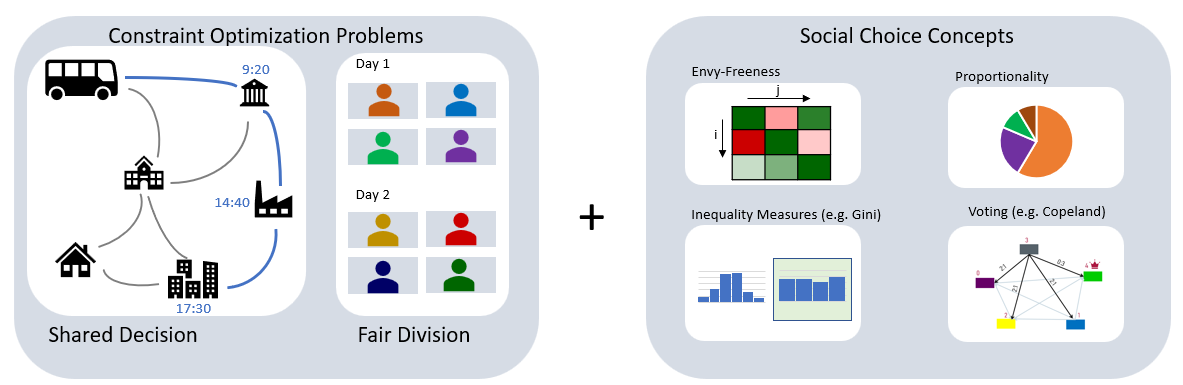
\includegraphics[width=\textwidth]{concepts}
    \caption{The components of algorithmically fair collective constraint optimization problems: Shared decision problems (e.g. one travel itinerary per group per day) or division problems (e.g., allocating desk seats subject to WFH constraints and mutual availability) are combined to a variety of social concepts.}
    \label{fig:overview}
\end{figure}
\chapter{Related Work}
Recently, algorithmic fairness has gained more attention. The need for fair and equal distribution of goods has been recognized. There are many different approaches to achieve these goals, such as those shown in \cite{.2022,FelixBrandtVincentConitzerUlleEndrissJeromeLangandArielD.Procaccia.}. Both of them focus on a wide variety of fairness metrics and explain why their result is sufficient for a fair allocation. \\Other literature focuses on very specific allocation problems, such as those discussed in \cite{Ala.2021}. The main focus in this work is the application of the whale optimization algorithm to an appointment scheduling allocation problem. \\The main focus of this work is on a general overview of fairness metrics and how they be combined depending on the structure of the allocation problem.\\  Besides the allocation problems being optimized there is also work on optimizing the metrics themselves to better fit a generous amount of real-world scenarios, such as the adaptation of voting theory to iterative voting as shown in \cite{Bhavnani.2022b}. 
\\ A rather new method to achieve fairness in a repeated allocation problem was shown by \cite{Elokda.2023}. Artificial karma is used as currency in an auction scenario to ensure that giving and taking is equally performed by the agents.
 \\Fairness literature is usually combined with game theory.
While game theory generally focuses on both, explaining an agent's past behavior and generating a module to describe the overall distribution of goods among a set of agents, this work focuses only on the second part. While it may be interesting to look for the reasons behind an agent's behavior, the overall goal is to obtain generic building blocks for allocating goods to the group of agents. Therefore, the focus is on the future allocation rather than analyzing the past.
\\Cooperative game theory shares some similarities with fair constraint optimization as its main focus is also to generate the best possible outcome for agents forming coalitions \cite{.2022}. In contrast to cooperative game theory, the considered agents do not form coalitions. Even though the considerations about artificial karma are quite close to cooperative game theory, this work does not focus on how to create the best coalitions, instead, each agent focuses only on its satisfaction scores. Nevertheless, agents can still use different strategies to generate the best possible outcomes. They can do this by adjusting their valuation functions and thus affect the overall outcome.
\chapter{Fundamentals and Background}
\section{Defintion of an Allocation Problem}
This section describes how an allocation problem can be defined and which components must be considered to ensure an optimized result.
\subsection{Resources and Agents}
A collective combinatorial optimization problem requires a defined set of resources, which may vary in type.  The set of resources does not need to be homogeneous. To interact with these resources (e.g. to receive, calculate valuation functions, or vote) a set of agents is required for the problem statement. These agents do not have to be persons, they can also be abstract groups or variables \cite{.2022, FelixBrandtVincentConitzerUlleEndrissJeromeLangandArielD.Procaccia.}. The resources do not necessarily have to be split between the different agents. The allocation problem can also be a shared decision. We therefore divide between these problems. \\More specifically, we first distinguish two different classes of collective combinatorial optimization problems, given by (typed) decision variables $X$, constraints $C$, and agents $A$ with utilities $(u_a)_{a \in A}$:

\begin{itemize}
    \item \textbf{Division problems} deal with the allocation of resources to agents, such as desk space in a shared office or charging time reserved for a particular EV. Formally, they can be characterized by partitioning of decision variables $(X_a \subseteq X) {a \in A}$ such that the utility of agent $a$ \emph{only} depends on the values assigned to the variables in $X_a$ -- without externalities. For example, given the same reserved desk slots, an employee is indifferent to the assignments of the other desks. Solution concepts include constraints for \emph{envy-freeness} or \emph{proportionality}.
    \item \textbf{Shared decisions} By contrast, here we need to make decisions on a shared set of variables that we cannot localize to a particular agent -- think of a shared itinerary in group travel where a group of 15 travelers must agree on 6 out of 15 possible sights and the order in which to visit them. 
\end{itemize}

Moreover, a distinction between \emph{single-shot} and \emph{repeated} interactions is useful in terms of fairness: In a single-shot decision, an overall trade-off between agent satisfaction (e.g., using the Rawlsian ``maximize the minimally satisfied'') and social efficiency (``highest average satisfaction'') needs to be found, explained, and justified. In a repeated interaction, there is a chance to compensate for past bad allocations (for certain agents) by giving them priority in future instances, as sketched out in \cite{.2022}.  Both division and shared decision problems can be repeated within the same group of agents: think of allocating desk slots over multiple days or weeks, or deciding an itinerary for each day of a week for the same group of travelers.

\subsection{Soft and Hard Constraints}
Each optimization problem deals with a set of constraints. They can be split into multiple categories. The first is hard constraints for all agents. These constraints must be achieved to generate a valid result. The constraints are set for all agents.\cite{.2022} \\If we consider an example of a group of 5 employees sharing an office with 2 tables and the urge to allocate the tables to the agents for a certain week, a hard constraint for all agents could be that one agent can only be mapped to one table per day and one table can only be mapped to one agent per day. There might also be cases where hard constraints are only dependent on a special agent. In the already given scenario, this could be one agent needing some hardware to work on which is located in the office and can not be taken home. A solution with no table allocated to this person on the days his work is dependent on the hardware is no valid solution. \\Next to these hard constraints there can be some preferences of agents. We will call them soft constraints as they benefit the solution if they are met but it is not necessary to follow them to get a valid solution. \cite{.2020,.2022} Soft constraints can again be divided into soft constraints for all agents and soft constraints for only a part of the agents. \\The allocation of tables in a shared office can also express soft constraints. For example in this scenario three agents are working on their own specific projects while two people work on the same project. Both of them want to attend in the office at the same time, to be able to discuss open topics in person in the office. If this request can be fulfilled the agents would value the solution more but a day with people from two different teams being in the office would still be valid. \\Single agents can also have preferences on when they want to work from home or in the office. These preferences are not the same for every agent and should still be covered as much as possible in the optimization process even though they are not necessarily met for all valid solutions. \cite{.2022}


\section{Main Concepts of Fairness}
\subsection{Utilitarianism}
Utilitarianism is an approach to defining fairness that emphasizes the importance of the solution with the highest total expected utility. Thus, maximizing overall welfare is necessary when using fairness as an optimization factor. The initial example of Utilitarianism was dealing with the distribution of wealth among a population. When considering the distribution of wealth with Utilitarianism, we must take into account each person's wealth (represented by $x_i$), as well as the utility derived from that wealth by the person i (represented by $u_i(x_i)$). The Utilitarian approach to wealth distribution entails maximizing the total utility of all individuals within the region of interest. To guarantee a suitable outcome, we must factor in a budget of $B$, with the sum of individual wealth restricted by this budget. \cite{.,XinyingChen.2023} Therefore a feasible means of mathematically defining fairness is:\\
\begin{align}
   max\sum_{i=1}^{n} u_i(x_i) \\ \sum_{i=1}^{n} x_i = B
\end{align}
\\ \cite{XinyingChen.2023}
By setting it in the context of medical health distribution as shown in \hyperref[sec:motivation]{Motivation} one can construct the following use case:\\ When presented with a triage problem at a hospital, $c_i$ denotes the measurable cost of an individual's treatment, while $x_i$ determines whether the corresponding agent will receive this treatment. To determine the potential success of the treatment, we will employ quality-adjusted life years ($a_i$) which represent the years that a patient is expected to live in perfect health, with their current health state. When treatment is given, this value increases to $a_i + b_i$. It is important to remember that the addition of $b_i$ can only be considered for those who receive the treatment, and not those patients not receiving the treatment. With these assumptions, we can develop a mathematical function to resolve the issue by accommodating the utilitarianism approach.\cite{XinyingChen.2023} \\
\begin{align}
  \underset{u,x}{max}  = \left\{ W(u)\ | \begin{array}{l}
    \sum_{i} c_i(x_i) \le B\\
    u_i=a_i + b_i x_i \ x \in \{0,1\}, all\ i
  \end{array}\right.
\end{align}
\cite{XinyingChen.2023} \\
The welfare function, denoted by $W_u$, can vary depending on the approach taken. For instance, it can be represented as the total sum of all $u_i$, or as a function that minimizes unfairness. 
The most appropriate welfare function should be selected based on the specific use case. \cite{XinyingChen.2023}

\subsection{Egalitarianism}
In addition to the concept of Utilitarianism another common method used to define fairness is Egalitarianism. The central argument put forth by John Rawls posits that the choice of the optimal solution should not be influenced by the decision maker and the ultimate aim is to maximize the outcome for the least advantaged. \cite{XinyingChen.2023,.} Therefore Egalitarianism is also called Rawlsian welfare in some cases. To arrive at this conclusion, Rawls envisions a scenario in which a group of individuals seeks to distribute a resolution of a fundamental need among themselves, with no knowledge of their respective positions in society. Therefore, proponents of Egalitarianism agree that the welfare of the individual in the worst situation should be maximized and that the distribution of goods should be tailored to their circumstances. Therefore the solution with the maximum of the minimum value is chosen when a given set of solutions is considered. \\
 \cite{XinyingChen.2023,.,FelixBrandtVincentConitzerUlleEndrissJeromeLangandArielD.Procaccia.} Egalitarianism is relevant for predictable outcomes, e.g. when basic needs must be met.\cite{.} However, if outcomes are uncertain, it may not be the optimal solution. The mathematical expression for fairness under Egalitarianism is: \cite{.}
\begin{align}
max\{ min\{u_i(x_i)\}\}\\
\sum_{i}u_i(x_i) = B\\
x_i>=0, all\   i
\end{align}
With max and min being maximization or minimization functions. $u_i$ being the welfare function of agent i and $x_i$ being the amount of good given to agent i. B is the budget.
\\In the example of distributing a limited amount of tables to a set of coworkers based on their satisfaction levels due to their preferences of working in the office or remotely, $x_i$ would represent the set of tables assigned to agent i, $u_i(x_i)$ would be the satisfaction of agent i when given the distribution of his tables during a week. The limitation of the budget: $\sum_{i}u_i(x_i) = B$ would need a change to $\sum_{i}(x_i) = B$ because in this scenario the satisfaction levels do not have a boundary but the number of tables which can be assigned to the agents have a physical limitation which has to be considered.
\\To show how egalitarian solution-finding works, let's assume an office with only two tables and five coworkers working in this office. A random assignment distributed three different solutions. The agents ranked the solutions on their satisfaction from 0 being the worst to 100 being the best. Let's assume the ranking of the agent is comparable by assuming a list of criteria to deviate the satisfaction amount. The outcome of the voting is the following:
\begin{itemize}
\item Solution 1: $agent_1$: 30 $agent_2$: 30  $agent_3$: 60 $agent_4$: 99 $agent_5$: 99
\item Solution 2: $agent_1$: 30 $agent_2$: 30  $agent_3$: 40 $agent_4$: 30 $agent_5$: 30
\item Solution 3: $agent_1$: 50 $agent_2$: 51  $agent_3$: 49 $agent_4$: 23 $agent_5$: 80
\end{itemize}
The Rawlsian principle now compares the minimum values:
\begin{itemize}
\item Solution 1: 30 
\item Solution 2: 30 
\item Solution 3: 23
\end{itemize}
Therefore the maximum of these minimal values is 30. The winning solutions would therefore be Solution 1 and Solution 2. Both these solutions are considered equal. To find one leading winner among this subset of solutions iterative Egalitarianism can be used.
\subsection{Iterative Egalitarianism}
Egalitarian welfare is only considering the maximization of the worst-off agent. The outcome of all other agents is not regarded in the solution path. Given several different solutions, there might be more than one with the best outcome for the one worst-off. To decide which of these solutions is the best, an iterative approach of Egalitarianism, often also called leximax welfare can be considered. This approach is sometimes also referred to as max–min fairness criterion \cite{.b}p.234. The main goal is similar to Egalitarian welfare. In the first iteration, the outcome of the least advantaged is optimized. This agent's value is then stored. No agent can get a lower value than the outcome of the first iteration. \cite{.b} In the second iteration, the second worst agent is searched for and maximized. Again this value is safed. Now in the third round, the third worst agent is searched for and maximized. The values of the worse agents still need to be equal to the values already discovered. With this criterium, all of the agent's values are optimized until everyone is getting their maximal values. \cite{.,FelixBrandtVincentConitzerUlleEndrissJeromeLangandArielD.Procaccia.,Chen.2020} \\The values could represent the amount of good given to the belonging agent but could also represent the agent's satisfaction values. Therefore the satisfaction of the one who likes the solution the least would be optimized, followed by the agent coming afterwards, etc. By optimizing the satisfaction value we can provide a fair solution.
\\Given the same example as shown in the previous section we were given the agent's satisfaction amounts:
\begin{itemize}
\item Solution 1: $agent_1$: 30 $agent_2$: 30  $agent_3$: 60 $agent_4$: 99 $agent_5$: 99
\item Solution 2: $agent_1$: 30 $agent_2$: 30  $agent_3$: 40 $agent_4$: 30 $agent_5$: 30
\item Solution 3: $agent_1$: 50 $agent_2$: 51  $agent_3$: 49 $agent_4$: 23 $agent_5$: 80
\end{itemize}
The first iteration would now be the same as explained previously.
The Rawlsian principle compares the minimum values:
\begin{itemize}
\item Solution 1: 30 
\item Solution 2: 30 
\item Solution 3: 23
\end{itemize}
This results in solution 1 and solution 2 as the approaches with the maximum for the worst-off agent. In the second iteration the worst satisfaction out of the set of solutions of the previous round is compared and the maximum of them is chosen:
\begin{itemize}
\item Solution 1: 30 
\item Solution 2: 30 
\end{itemize}
Again it is the same amount for both solutions. Iteration 3 searches for the next worst agent which results in the set:
\begin{itemize}
\item Solution 1: 60 
\item Solution 2: 30 
\end{itemize}
Now the worst-off agent in Solution 1 is higher than in Solution 2. Therefore solution is considered the best solution. If there are more solutions or Solution 1 would not be the only one left in this scenario, we had to iterate 5 times to get a set of solutions as winners. If there is more than one winner, the solutions are equal. In this scenario Solution 1 is the only winner. \\Iterative Egalitarianism therefore searches for the set of the best solutions for every agent being part of the allocation problem.

\subsection{Limits of Utilitarianism and Egalitarianism}
Both Utilitarianism and Egalitarianism, as expounded in the preceding sections, rely on predictable outcomes. If the outcome is not predictable the best solution can not be found. Furthermore, the second constraint of both approaches is their presumption that in the event of distributing goods, every individual requires and desires the same, and therefore, the maximum quantity of feasible goods. \cite{.,XinyingChen.2023,Bhavnani.2022b} Nevertheless, this does not always represent the situation. When considering a situation where multiple small companies share their packaging machines in a shared factory, it is important to recognize that the small company producing only two packages per day may not require the same amount of packaging time as a larger company. Therefore, it is important to acknowledge that the requirements of different actors can vary and may not be directly comparable. \\The two concepts represent different categories of fairness metrics. Utilitarianism is about the maximization of the overall efficiency while Egalitarianism focuses on the maximization of one agent's satisfaction. As both theories are not always relevant to every real-life problem, the next sections focus on other metrics to achieve either of both goals.


\section{Voting Theory}
Due to the limitations of utilitarianism and egalitarianism discussed in the preceding section, voting theory can be considered in scenarios where actors have different needs. The central idea of voting theory is that each actor possesses equal voting power, rendering the outcome fair as everyone has equal influence. The theory of voting relies on ordinal valuations, whereby solutions can be ranked according to certain valuation functions. \cite{Bhavnani.2022b}   Therefore, voting theory shares the same limitation as utilitarianism and egalitarianism, in that it is unsuitable for unpredictable outcomes. However as the ordinal ranking is not influenced by the valuation functions of other agents, their order is comparable even if different valuation functions were used \cite{Bhavnani.2022b}. Voting theory in general is the sum of all metrics used to empower people to vote for their preferred solution. \cite{FelixBrandtVincentConitzerUlleEndrissJeromeLangandArielD.Procaccia.} Therefore they are suitable for combinatorial optimization problems as the amount of outcomes is limited and agents can vote for their favourite outcome. \\As there are many different possibilities on how to evaluate the winner of a voting scenario the following chapters will highlight different social choice functions to determine the winner of a set of solutions by voting mechanisms. The precondition of this set of solutions is, that hard constraints were already taken into account in the generating process of the considered subset of solutions.  The characteristics of a social choice problem consist of the following items: 
\begin{itemize}
  \item solutions/alternatives s to choose from
  \item agents A
  \item linear ordering of every agent to every solution:  $x>^\mu y$
  \item ballots b to store the ranking of alternatives 
\end{itemize}
\begin{figure}[h]
\centering
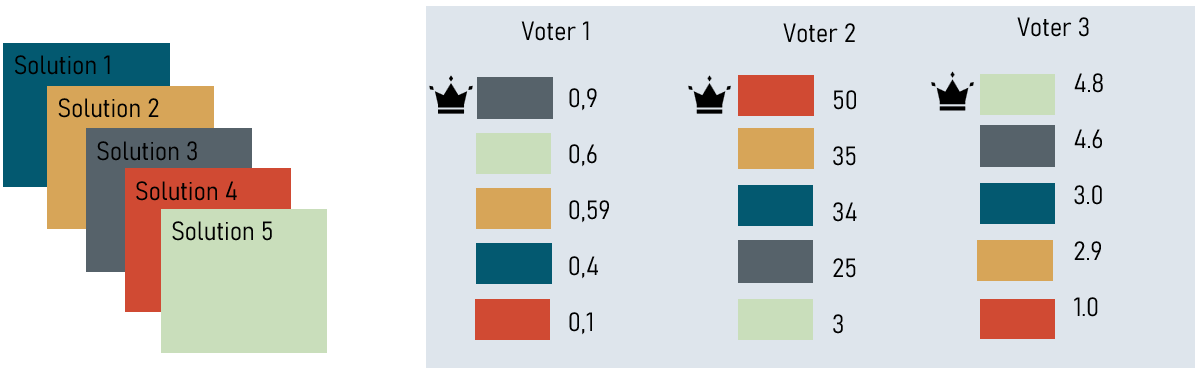
\includegraphics[height=3.4cm]{Voting_setting}
\caption{characteristics of voting setting}
\end{figure}
Different metrics specify the way this linear order is characterized. Some mechanisms require strict preferences while others work with ties and accept equal valuations among the solutions. The given problem to solve can therefore be an important indicator of which mechanism to choose.\cite{FelixBrandtVincentConitzerUlleEndrissJeromeLangandArielD.Procaccia.} If the chance of ties between the ranking of one agent and multiple solutions is likely, a metric that can handle these ties should be chosen.
\subsection{Plurality}
The first approach in voting theory to be mentioned is plurality voting. The mechanism is relatively simple to describe. The voters rank the solutions from the one they like most to the one they like least as shown in the overview in Figure 4.1 before. These rankings of each agents are called ballots \cite{FelixBrandtVincentConitzerUlleEndrissJeromeLangandArielD.Procaccia.} The number of voters with the same ballot is counted and the highest alternative within the ballot with the most votes wins, regardless of the other rankings in the ballot. \cite{FelixBrandtVincentConitzerUlleEndrissJeromeLangandArielD.Procaccia.} To give an example of plurality the example of the characteristics of voting theory in general is expanded by a higher amount of voters (630 in sum). The voters choose their preferred orders which leads to alternatives 1, 2, and 3. Each of these alternatives has a certain amount of voters which is denoted on top of each alternative in the overview.
\begin{figure}[h]
\centering
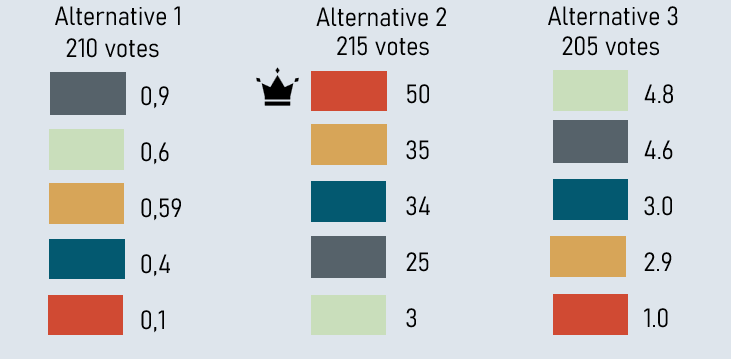
\includegraphics[height=3.4cm]{Plurality}
\caption{Example Plurality, original graphic at \cite{FelixBrandtVincentConitzerUlleEndrissJeromeLangandArielD.Procaccia.}}
\end{figure}
In this scenario, the second ballot and therefore the red solution would win. But the example also shows, that 415 voters ranked the red solution as their least favorite. It still wins plurality voting as it is the alternative with the most votes.
\\
This effect of plurality voting was also discovered in multiple real-world scenarios e.g. conservative Republican Alfonse D’Amato’s 1980 U.S. Senate winning in New York (a predominantly liberal state), with 44.88\% of the vote against democrat Elizabeth Holtzmann (43.54\%) and liberal Republican incumbent Jacob Javits (11.05\%).\cite{FelixBrandtVincentConitzerUlleEndrissJeromeLangandArielD.Procaccia.}
\subsection{Majority}
Majority voting is very similar to Plurality voting with one major limitation. The number of votes for the solution must be over 50\% of all votes. It is used in politics in different countries when the decisions are of the highest interest. The sum of the percentage of votes for the leading solution has to be at least 50\%.\\  In the above scenario, none of the alternatives would win as it takes at least 316 votes to be the majority. None of the alternatives exceeds this number of votes. \\Both Majority and Plurality voting are frequently used to convert voting percentage into seats inside a parliament \cite{Blais.1988} The need for more than 50\% of the votes in Majority voting can lead to a cluster of different parties being the government inside the country. This can be an advantage or a disadvantage when applied to an underlying scenario. \\One of the weaknesses of Plurality and Majority voting is the consideration of the interests of the minorities within the group of agents. \\To ensure fair voting the mechanism of Copeland and Borda are regarded in the next sections.
\subsection{Copeland Voting}
One of the most common social choice functions is Copeland voting.  Instead of the algorithms shown so far Copeland is relying on pairwise duells. With the Copeland voting mechanism the number of wins is counted and compared between the different possible solutions. The weight of the wins or losses and therefore the number of people voting for alternative 1 over alternative 2 is not taken into consideration. \cite{ALEXANDERJOHANPHILIPPEEK.2022,FelixBrandtVincentConitzerUlleEndrissJeromeLangandArielD.Procaccia.}  \\There are two different approaches of Copeland Voting: symmetric and asymmetric voting. The main difference is the way the Copeland values are calculated. While symmetric Copeland voting considers wins and losses, asymmetric voting only counts the number of wins for a certain agent.
\\The mathematical expression of symmetric Copeland voting is: \cite{FelixBrandtVincentConitzerUlleEndrissJeromeLangandArielD.Procaccia.}
\begin{align}
Copeland_{symmetric}(x) = \left| \left\{ y \epsilon S \left| x>^\mu y \right\} \left| - \right| \left\{ y \epsilon S   \right| y>^\mu x   \right\} \right|
\end{align}
\\According to the definition of asymmetric Copeland voting it can be expressed as:
\begin{align}
Copeland_{asymmetric}(x) = \left| \left\{ y \epsilon S  x>^\mu y \right\}  \right|
\end{align}
With S being the set of solutions and x and y being different solutions.
\\Using the distribution of goods among a specific number of actors as an example, the foundations of the Copeland voting mechanism can be described.  Firstly, a set of all possible solutions is created using basic statistical mathematics. Next, each actor can vote for their preferred solution, generating an ordinal set of solutions for every actor in the example. The ranking process itself is not specified in this step. Hence, a prospective voter could evaluate the solutions by determining their associated costs. Accordingly, the solution receiving the highest numerical value would be considered the least desirable. Another viable option is calculating the benefits of each solution, whereby the highest number represents the best solution. By not requiring the specification of an individualized voting approach for each voter, but only relying on the resultant ordered list of potential solutions, this method provides numerous customized possibilities for diverse stakeholders and is not dependent on comparable agent's valuation functions. After each actor has created an ordinal list of solutions, they are granted equal voting power for the next step. The various solutions are then compared to one another through a one-by-one approach in which two solutions are compared by reviewing each voter's ordinal list. \cite{Bhavnani.2022b, FelixBrandtVincentConitzerUlleEndrissJeromeLangandArielD.Procaccia.} When comparing solutions 1 and 2, solution 1 receives a point for every voter who prefers it over solution 2. The same method is applied in favor of solution 2. In the next step, the number of defeats is subtracted from the winning number. This step is not taken into account if the asymmetric approach is chosen. This process is repeated for every possible set of duels within the set of solutions, and the number of winning (and losing) duels is recorded for each possible solution.  In the end, each solution is compared based on points and the solution with the higher score wins the duel. Finally, the solution with the highest number of wins (and the lowest number of losses) is deemed the overall winner and is considered the fairest solution for all parties involved. In symmetric Copeland voting this is achieved by counting the number of wins and losses and subtracting the number of losses from the number of wins. The higher this value gets, the higher the number of wins was compared to losses. \cite{Bhavnani.2022b,.2022, FelixBrandtVincentConitzerUlleEndrissJeromeLangandArielD.Procaccia.}
The asymmetric Copeland voting mechanism can deal with ties among the different solution approaches. One possibility is not giving points to any of the alternatives while it is also possible to give each alternative 0.5 points for a tie. \cite{FelixBrandtVincentConitzerUlleEndrissJeromeLangandArielD.Procaccia.}
\begin{figure}[h]
\centering
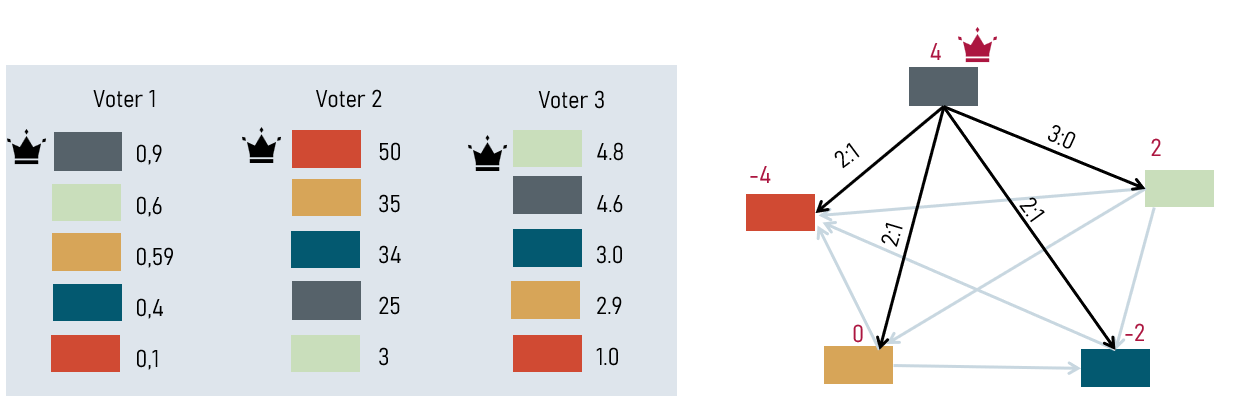
\includegraphics[height=4.4cm]{Copeland}
\caption{Example for a symmetric Copeland voting. The blue solution would be the winner with 3 wins and a copeland value of 3}
%\end{figure}
%\begin{figure}[h]
%\centering
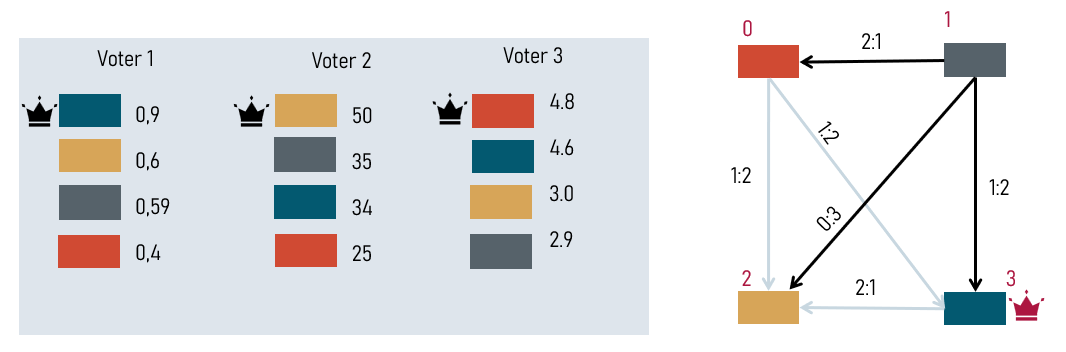
\includegraphics[height=4cm]{Copeland_asym}
\caption{Example for an asymmetric Copeland voting. The blue solution would be the winner with 3 wins and a Copeland value of 3}
\end{figure}
As an example of symmetric and asymmetric Copeland voting, we consider the voting prerequisites previously shown. With this chosen example the different calculations of asymmetric and symmetric Copeland values can be shown:
\\Even though in both examples blue is the overall winner as it is leading against all other alternatives, it shows the different calculation of the Copeland scores. While in symmetric voting the red solution is getting a score of -3 it is getting a 0 in symmetric voting. Also, the differences between the Copeland scores are much smaller in symmetric voting.
\subsection{Borda Voting}
Borda voting shares a lot of similarities with Copeland voting. The main difference is the consideration of weights in the Borda voting mechanism. Copeland counts the number of wins (and losses) while Borda calculates the weight differences. \cite{FelixBrandtVincentConitzerUlleEndrissJeromeLangandArielD.Procaccia.}Therefore a defeat of a pairwise duel of two very similar solutions does not get as much power in the resulting score as a loss of very different solutions would. The weights compared in Borda voting are usually the number of voters preferring one solution more than the compared one. 
\begin{figure}[h]
\centering
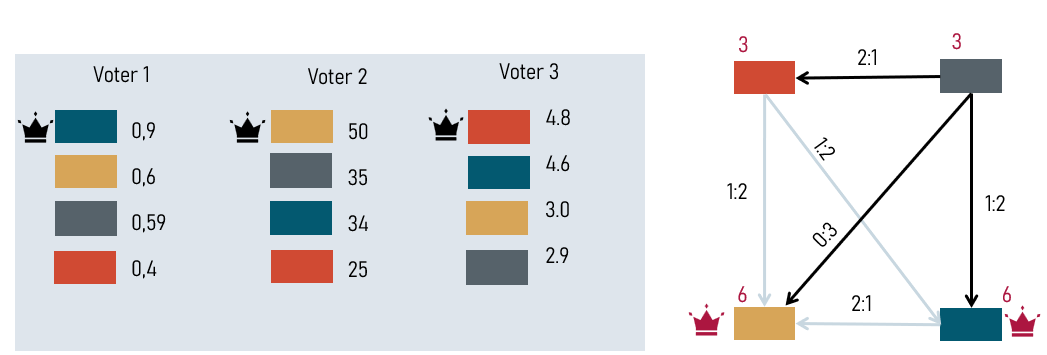
\includegraphics[height=4cm]{Borda_asym}
\caption{Example for an asymmetric Borda voting. The blue and yellow solution would be the winners with a Borda value of 6}
\end{figure}
\\The example shown in Copeland voting can be applied to Borda voting. With the same set of agents, the result is different. In Copeland voting the blue solution was the only winner while in Borda voting blue and yellow are equal results of the asymmetric Borda voting. As Copeland, Borda voting can be differentiated into symmetric and asymmetric approaches. The symmetric one considers both wins and defeats while the asymmetric approach is only considering the number of voters voting for solution 1 over solution 2 to achieve the Borda value. \cite{FelixBrandtVincentConitzerUlleEndrissJeromeLangandArielD.Procaccia.}
Even though Copeland and Borda voting share the same problem of missing minorities' interests within the overall outcome like Plurality and Majority voting they might lead to different results. In contrast to the voting mechanisms Plurality and Majority voting, they also include the voting of the ballots that do not obtain the majority. 
\subsection{Iterative Voting Theory}
The limitation of the above-explained voting mechanism is given when observing a high number of different solution possibilities. Because of the pairwise tournaments in Copeland and Borda voting the number of calculations to get the winner is increasing exponentially. Due to the high calculation effort, there is a need to search for more efficient ways to implement Copeland or Borda voting without the risk of getting too high calculation times. \cite{Bhavnani.2022b}
\\One approach to solve this issue is a sampling-based algorithm as shown in \cite{Bhavnani.2022b}. Therefore the solution pool is not considered as a whole but only a few samples are taken out of it. The voting mechanism like Borda or Copeland is now calculated based on this subset of solutions. Only the winning solution is kept and in the next iteration, new samples are compared to this solution. To minimize calculation time and costs this procedure can be stopped before all solutions within the solution pool are considered. This makes this approach very sensitive to the sampling set of the solutions. When compared to only bad solutions the one which is the best among them might seem good when in reality there might be way better options in the overall pool. \\One possibility to face this issue is choosing samples that differ the most. The samples chosen from the pool of solutions therefore should not be similar to each other. By using the example of shared office desks among a group of agents the solutions in the pool represent different seat assignments. Therefore when comparing only a few samples they should not represent a set of solutions where one agent changes for desk A while all other agents stay the same on every other desk. The variance of these solutions is quite low as only one agent changes even though the solutions are part of the solution pool. The better alternative would be to compare completely different sets of seat assignments where e.g. at the first iteration no two agents can be assigned to the same desk in two or more sample solutions. Of course, this solutions can be added in the next iteration to encounter the best solution.
\begin{figure}[h]
\centering
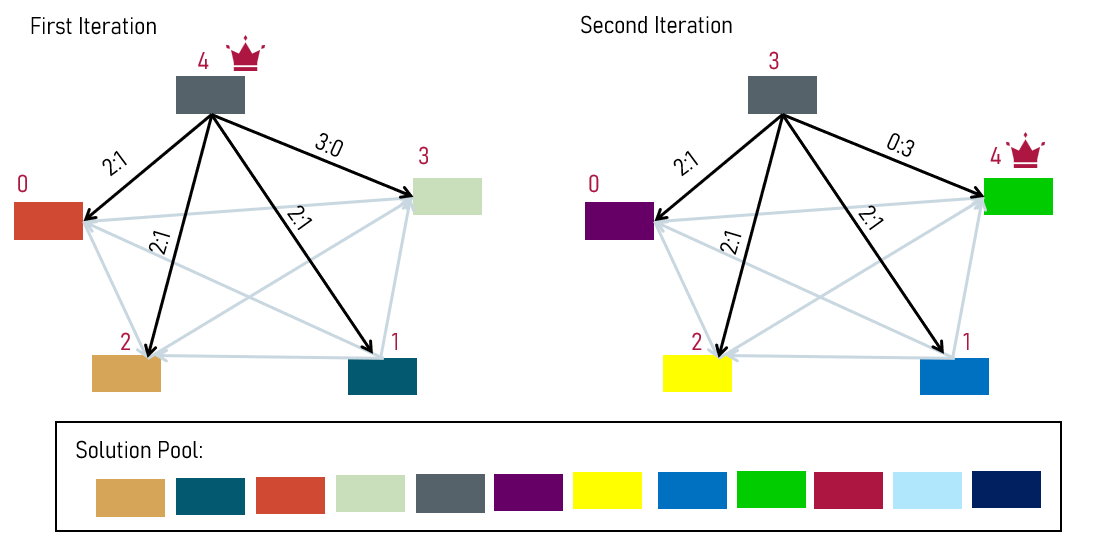
\includegraphics[height=6cm]{Iterative_voting}
\caption{Example for iterative Copeland voting. The grey solution would be the winner with 4 wins in the first iteration while compared with 4 new solutions green is the competing winner.}
\end{figure}
Figure 4.6 shows an example of iterative voting. The solution pool covers 12 different solutions. Out of these 12 solutions 5 samples are chosen. The asymmetric Copeland tournament is now performed using these five solutions. The winning node grey is now taken and new samples from the solution pool are compared. The next asymmetric Copeland tournament is the second iteration. In this tournament, the green node is winning and therefore replacing the grey node. Please note that there are only 12 solutions to make it easier to show the principle of iterative voting. In reality, 12 solutions might still be calculable. Instead of Copeland tournaments Borda voting could also taken into consideration to find the most suitable solution.











\section{Fair Maximization of Agents Satisfaction}
\subsection{Envy-Freeness}
In most real-world scenarios, agent's preferences are not comparable.
Due to this incomparability of the valuation of different agents, it is useful to not compare the outcome of different utility functions as values themselves but as ordered ranking given to the different solutions by the agents. We have already seen this concept of ordered rankings in voting theory. Another fairness metric using this concept is Envy-Freeness. Envy-Freeness is given if the valuation function $V_i$ for every agent i is scoring the highest result with their allocated resources when compared to every other agent's resources. Therefore Envy-Freeness is used if the allocation problem is a division problem where every agent is assigned a set of resources.
According to a valuation function:
$X \succeq_i Y \leftrightarrow V_i(X) \geq V_i(Y)$
Envy-freeness is defined as: There are no agents $i$ and $j$ such that
$V_i(X_i) < V_i(X_j)$
with $X_i$ and $X_j$ being the allocated values for agents i and j.
Therefore the pool of solutions given by the problem shape and some hard constraints are calculated and afterwards, envy-freeness is calculated. An envy-free solution can be considered a fair solution as there is no allocation to another agent j that agent i would prefer. \cite{.2022,FelixBrandtVincentConitzerUlleEndrissJeromeLangandArielD.Procaccia.} When Envy-Freeness is considered as fairness metric some other optimizing value like the maximization of the overall value should still taken into account as an allocation of 0 to every agent would be considered a valid solution in the case of envy-freeness. \cite{Bouveret.11222023} In most real-life scenarios this would not be a suitable solution as the whole optimization would not be relevant.
\\If there is no envy-free solution besides every agent getting 0, the given constraints can not lead to a completely fair solution when envy-freeness is chosen as a metric of fairness. \\When dealing with a limited amount of agents it can be useful to display an envy-matrix as shown in Figure x. Therefore the results of the different agents' valuation functions can be compared. The diagonal in the matrix represents the result of the valuation function of agent i with its allocated values. In the shown matrix this is equal to agent i and agent j referring to the same agent. If this number is the highest for every agent the distribution would be considered an envy-free solution. If not, the combination of multiple matrices can show that envy-freeness is not possible to achieve and generate the output with the least envy. It therefore offers a transparent decision and ensures that all agents see the impact of their soft constraints in the result.\\ 
\begin{figure}[h]
\centering
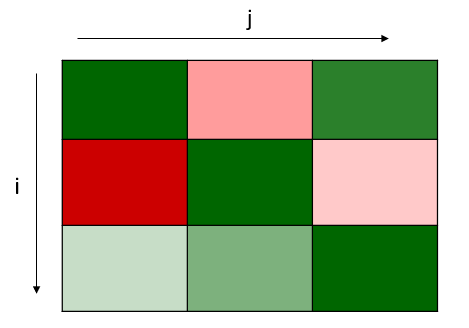
\includegraphics[height=6cm]{envy_matrix}
\caption{Example of a matrix showing envy-freeness. Dark green represents the highest number, while dark red represents the smallest number.}
\end{figure}
The result of the envy-free algorithm can be no solution,  exactly one solution, or a set of solutions where no agent prefers another agent's allocated goods. When a set of solutions is returned it is still possible to choose the result with one other fairness metric of social efficiency in this chapter.
\subsection{Proportionality}
The concept of proportionality also deals with the satisfaction of all agents regarded as single agents and not compared with each other's valuations. The aim is to achieve a proportional allocation based on the maximal achievable valuation per agent divided by the number of agents in the allocation process. To calculate the maximal achievable valuation per agent the allocation problem is regarded as if the agent would be the only agent in the scenario. \cite{FelixBrandtVincentConitzerUlleEndrissJeromeLangandArielD.Procaccia.} The maximal achievable valuation per agent is limited by hard constraints of the overall problem and soft constraints of every agent. Therefore the maximal achievable valuation does not necessarily have to be the maximum of the valuation function. The proportionality concept is usually used for cake-cutting division problems. If an agent just wants as much of a cake shared with 3 other agents as possible, it would be considered fair if each of them got at least one-fourth. \\The same concept can be portrayed in more complex scenarios like a shared office situation. Let`s assume an agent $agent_i$ who wants to come to the office to an allocated seat every weekday of the following week but has to share the office with 4 other agents and the office consists of only 2 tables. His utility function is a sum of assigned seats with each assigned seat representing a value of one. The only hard constraint in this scenario is that an agent can not be assigned to two or more tables on the same day and no two agents can be assigned to one table on the same day. Therefore the maximum of his valuation function is 5.  Regarding proportionality, it can be considered fair if his utility function is equal to one. Therefore if he is assigned to at least one table for this week the solution is considered fair for $agent_i$ if proportionality is chosen as fairness metrics. \\By expanding this scenario to all other agents having the same utility function as the one already explained, the principle of super-proportionality can be achieved. In this scenario, we could allocate each agent to two tables per week resulting in a utility function of 2 for every agent. As this is higher than the proportional value every agent wanted to get, this is an optimal solution. Those cases are called super-proportionality. In real-world scenarios, this is not always achievable and highly dependent on the given task. \\The outcome of proportional optimization can be zero, one, or multiple possible solutions. The metrics of fair overall efficiency can then be used to choose the best solution within the set of suitable ones. 

\section{Statistical Measurements}
\subsection{Gini Coefficient}
Overall efficiency can be provided when the Gini coefficient is considered as an optimization metric. The Gini inequality index is usually used to calculate the disparity of distribution. This originates in the initial use of the Gini coefficient for income inequality \cite{.2022}. 
The Gini index is defined as: 
\[
  Gini(x) = \frac{\sum_{i=1}^n \sum_{j=1}^n | x_i - x_j| }{2 n \sum_{i=1}^n x_i} \cite{.2022}
\]
One of the restrictions of the Gini index is its limitation to positive input values. Therefore the outcome is always standardized between 0 and 1. \cite{ALEXANDERJOHANPHILIPPEEK.2022} 0 represents perfect equality while 1 is the distribution to one agent only and all others not receiving anything.\\
When considering Utilitarianism and Egalitarianism as our underlying concept of fairness it makes sense to use Gini inequality to calculate if the good is fairly distributed among the set of agents. The basic concept is that every agent wants as much of the given resource as possible and therefore it can be considered an equal solution if everyone gets the same amount of goods. \\When focusing on more complex scenarios the pure distribution of the goods does not seem to be the most preferable approach. \\ Let's assume an office situation where agents can register to apply for tables for each day of the week. When Agent A wants to come into the office 2 times a week and gets distributed to 4 tables a week and Agent 2 wants a table on every day of the week and also gets assigned to 4 tables, the solution would not be considered fair for the agents. Agent 1 must come to the office on two more days as he wants while Agent 2 does not have the option to come in on all 5 days even though the perfect preferred solution might be a possible option. Even if Agent 1 is not forced to come to the office if assigned to a seat, the solution is not ideal. The Gini inequality index can still be used in this scenario if we do not apply it to the distributed good but to the satisfaction level of every agent. Therefore a fair solution is a solution with equal distributed satisfaction among the agents. In the shown distribution with 4 tables, every agent getting the same amount would not be considered fair as the satisfaction level of the agent with 1 more table than requested might be higher than the one with one less table (as the first agent could still just not attend the office on all his days). Therefore Gini inequality index can be used to calculate a value of the disparity of fairness and therefore be a good indicator of how fair the resulting solution is. This resulting set of solutions should be optimized by different other metrics to ensure the maximum of equal fairness. Of course, other metrics as the maximal use of all given goods should be optimized at the same time as the distribution of 0 to all agents ensures an equal satisfaction factor but can not be seen as the optimal solution. Like Utilitarianism and Egalitarianism Gini index also deals with the comparison of agents' valuation functions with each other. If this is not suitable to the given scenario other fairness metrics should be chosen.
\subsection{Variance of Agents Satisfaction}
Another metric of dispersion, similar to the Gini Index, is called Variance. It represents the difference in the distributed values.  The higher the difference in the result values, the higher the variance. Therefore it can be used to describe not only dispersion but also the fairness and equality of an allocation problem. As seen before in most real-world scenarios equal distribution is not necessarily the fairest solution. Therefore instead of taking the different distributions and calculating the variance out of it, it might seem as a better approach to use agent satisfaction instead. Therefore the main goal is not an equal distribution of the belonging good but an equal distribution of satisfaction among the agents. \\One of the most important things to keep in mind when using variance as a fairness metric is its need for a second optimization factor. In the case of satisfaction values being equally distributed, the goal also needs to be a maximized distribution of the given good. Therefore we exclude the possibility of assigning no goods to all agents which would consequently still lead to an equal distribution and low dispersion. \cite{.2022} \\Variance can be calculated as the quadratic difference of the arithmetic means leading to the following equation:
\begin{align}
variance=\frac{1}{n}\sum\limits_{x_i\in N} (x_i-\overline{x})^2.
\end{align}\cite{.2022}
With N being the number of agents. In most cases, variance and standard deviation are used with each other as standard deviation is the square root of variance. It can be seen as the average difference from the mean of the values. Therefore we can again use it as fairness metrics if the value we analyze is the satisfaction of the agents and we consider an equal distribution of satisfaction as fair. The lower the standard deviation the closer the satisfaction factors are to each other. As seen with variance the need of a second attribute to maximize the satisfaction is again required.
\begin{align}
standard_deviation=\sqrt{variance}=\sqrt{\frac{1}{n}\sum\limits_{x_i\in N} (x_i-\overline{x})^2.}
\end{align}
\cite{.2022}

 \subsection{Maximal Product of Agents Satisfaction}
Another way of finding equal results is based on a geometrical concept. The product of two numbers is the highest if the difference of the numbers is small. This leads to the maximum of the product of two numbers being the distribution of both numbers where both are closest to each other and therefore equalized. \\The proof of this theorem can be visualized when looking at the graphical plot of the product of two numbers x and y. 
\begin{figure}[h]
\centering
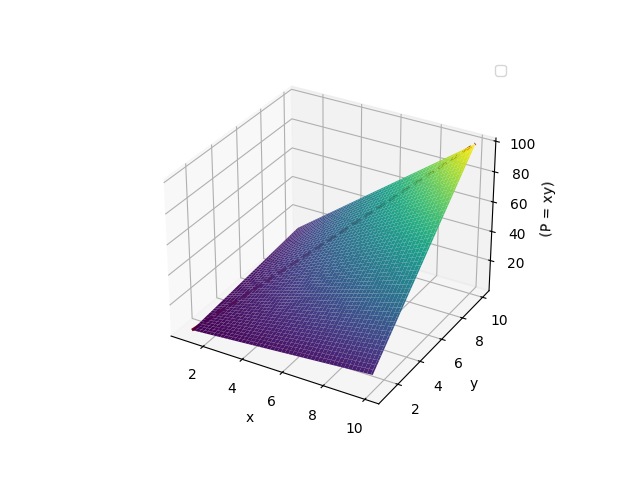
\includegraphics[width=1.0\textwidth]{x_times_y}
\caption{The plot shows the product of x and y both within the ranges of 1-10. The highest point is achieved when x and y are equal to ten. The line from (0,0,0) to (10,10,100) is the line with the maximum height for the given values.}
\end{figure}
\\Therefore equal and fair distribution can be achieved if the product of the valuation function of agents is maximized. (Marl-book)
\\Even if the sum of both values is limited, the highest number of the product is still achieved if the two numbers differ the least. A way to express fairness can therefore be shown by the maximization of the product of all agent valuations. \\As seen previously if fair allocation is not equal to equality within the allocation of the goods, the agent's valuation functions should be equalized instead of their distribution. Therefore this theory focuses on an equal distribution of the resource by maximizing the product of all utilities. \\This metric can easily be combined with other metrics like Utilitarianism. In this case, the maximum of the sum of the valuation functions and the maximum of the product of the valuation functions is searched for. (Marl-book)

\section{Repetition}
Fairness in resource distribution is about ensuring that agents facing similar needs receive comparable access to limited resources. Sometimes this is not achievable during a single allocation. Therefore the goal can be balanced across multiple iterations of allocations if the problem exists more than once.\cite{Elokda.2023}
\subsection{Artificial Karma}
When the allocation process does not only take place a single time but is repeated multiple times we can also think of a new metric realizing the balance between the allocations. One of these approaches is the use of artificial karma. It is inspired by the Indian tradition of karma. The main concept is based on the way small communities share a limited amount of resources like fish in a lake \cite{.c} \\The principle shown in \cite{Elokda.2023} is based on a situation where an indivisible good should be allocated to one of two agents randomly picked out of a bigger set of agents. This procedure is repeated infinite times. One example of such a situation is a car ride scenario where two people are requesting a car ride but there is only one car available at this time. This situation is taking place more than one time. The agents may have different preferences during the time sequences and can show their preferences using their karma scores. Karma therefore is treated as a counter of taking or giving. If an agent is not taking the resource in a one-to-one tournament it will increase his karma score and the agent might benefit from the higher karma score during the next round. Once an agent takes the ressource it will decline its karma score so the probability of this same agent getting the next ressource as well is limited. Therefore an agent with a high karma score has probably not taken many resources in the past while an agent with a low karma score has probably already taken a higher amount of resources. Consequently, the main focus of artificial karma is on alternating the allocation of goods among the agents.  The amount of karma given or taken by the agent does not need to be the same for every tournament. It can differ by the preferences of getting the resource to the given time. The karma allocation can therefore be seen as a kind of public sale. With this technique, it is possible to include the agent's preferences. \\Karma is therefore a measurement of how much the agent needs the current distribution. Unlike other fairness metrics, the agent's valuation is therefore comparable because it is based on the number of karma they are willing to invest. \\The reason money and karma need to be split is because of the uneven distribution of money in the first place. If the distribution of goods were a public sale for all goods, wealthy people would always have the privilege of more prospects towards resources. Karma on the other hand can be equally distributed at the beginning of the scenario and afterwards, it is always based on the resources taken or given and therefore guarantees that there is no overly favored agent getting all the resources. If an agent spends too much of his karma there will be no karma left for the next rounds etc.  \cite{Elokda.2023}
There are different approaches to how much karma is taken from and given to certain agents. This work focuses on the approach called "Pay bid to peer". In this approach the one bidding the higher value is directly transacting the money to the one not getting the resource. \cite{Elokda.2023} \\Given the above example of two agents "fighting" for a car ride. Let's assume both agents are new to the platform of the taxi company so their initial karma level is both 100. The taxi company would now offer the agents to set the amount of karma they are willing to spend on the car ride. The agent getting the car ride is subtracted from the amount of karma while the one not getting the car ride is gaining the amount of karma to their account. When the agent not taking the ride is requesting a new one he has more karma to spend and therefore it is easier for him to get the new car ride. The bidding process does not necessarily need to be done by the agents themselves. There could also be some kind of optimization algorithm training on how much karma to invest to get the best-case scenario for the given agent.
\\Even though the process of getting or not getting a ressource at one iteration might seem unfair to agents it can be balanced out over multiple iterations. Artificial karma is a better approach than money to reach that goal of balancing multiple iterations of allocations as it only relies on giving or taking and can be evenly distributed in the first place. \cite{Elokda.2023}

\chapter{Usage of Metrics based on Problem Characteristic}
The following chapters divide real-world situations of fair allocation of a set of resources among a set of agents into eight categories. The categories are explained and the metrics used for these kinds of situations are explained and adjusted to the type of problem.
\begin{figure}[h]
\centering
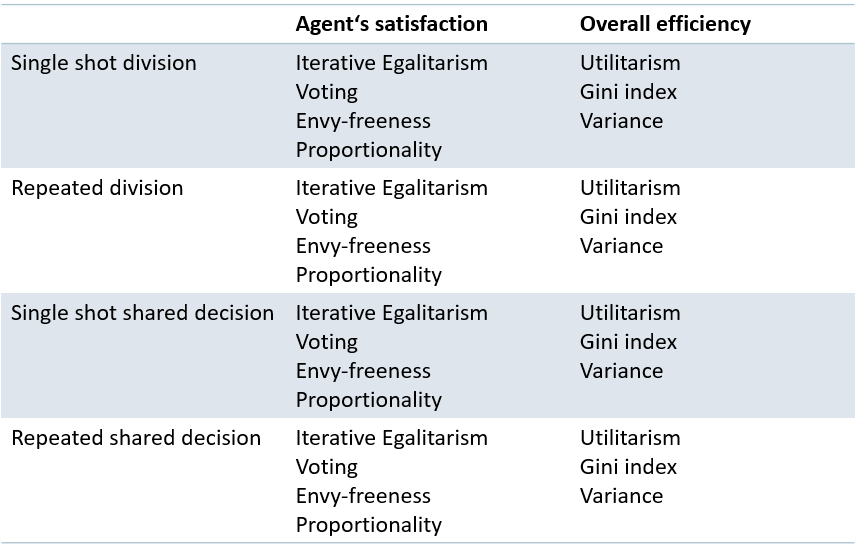
\includegraphics[height=10cm]{Categories}
\caption{Overview of the categories to be explained with real-world scenarios in the next chapter. Some metrics are doubled in the list but there application needs to be adjusted based on the problem's characteristic.}
\end{figure}
\section{Single-shot Division Problems}
Single-shot division problems are situations consisting of a set of agents and a set of resources distributed among these agents. The agents are assigned a set of resources without the resources being shared by multiple agents. In some use cases, the resources can be split and therefore assigned to more than one agent. To still be considered a division problem there must be the possibility of agents getting different sets of resources. Therefore the agents do not have to agree on one common solution in division problems. The metrics used for this kind of problem are
\begin{itemize}
  \item Utilitarianism
  \item Egalitarianism / iterative Egalitarianism
  \item Voting
  \item Envy-freeness
  \item Proportionality
\item Gini
\item Variance
\item Product of Agent's satisfaction
\end{itemize}
The metric to be chosen from the list is dependent on the given scenario and the definition of fairness or equality. Even within the group of single-shot division problems, we can divide the scenarios into multiple different groups. One of the main differences within the scenarios of single-shot divided problems is the goal of the distribution. Is fair overall efficiency or the maximization of agents' satisfaction the main focus of the distribution? Depending on this question different metrics need to be considered to ensure fair allocation. If the overall efficiency is the main goal one agent's preferences do not necessarily need to be met to achieve this goal. Suitable metrics are Utilitarianism, where the improvement of the overall welfare is the main optimization factor, and the Gini coefficient ensuring equal distribution. If the agent's satisfaction is the main goal, metrics like iterative Egalitarianism, voting, envy-freeness, and proportionality should be taken under consideration as they focus on the agent's preferences instead of the overall welfare. Voting is considered an agent's satisfaction measurement as it highly relies on the agent's preferences instead of an overall equality approach. This classification is based on the assumption that agents only consider their allocation in voting theory. Therefore two solutions with the same allocation for one agent need to be ranked the same in the used voting technique.\\ Furthermore the resources can be separated into two categories: divisible and indivisible. Divisible resources can be split, like time or money, while indivisible resources can not be split like tables in a shared office. It does not make sense to let two agents sit at the same office table at the same time. Even though divisible resources can be split, in single-shot division problems usually all agents still get a unique set of non-shared resources. The amount of money or time given to them does not need to be shared with other agents. Therefore the next two subsections will not differ for divisible and indivisible resources.

\subsection{Agent's Satisfaction}
As one example of a single-shot division problem focusing on agent satisfaction, we want to focus on an indivisible resource allocation issue.
Indivisible resources can not be split into more items. One scenario would be a single desk-sharing scenario. Let's assume a group of coworkers usually working at workplace B wants to visit workplace A for a single day. Because of some limitations to workplace A, there are currently only 2 desks available. Therefore only 2 agents get the chance to visit workplace A and are therefore assigned to one of the tables. In this scenario, it is not practical to split the desks in some matters like "agent 1 can get the table from 8-10, agent 2 from 10-12, etc." because the agents do not have a place to work remotely if not assigned to a certain desk. Therefore the desks can not be split. On the other hand, we can not assume that every coworker wants to visit workplace A at this time and an allocation of the seat is the best outcome for them. Therefore we need to ask for preferences among the agents. These preferences or soft constraints could consist of different approaches e.g. if the day is suitable for them but could also have connections to each other e.g. agent A and agent b working on the same project at the moment and need to communicate a lot during office hours. Therefore both of them either want to travel to workplace A together or none of them. The main goal is to find a fair allocation of the two tables among the coworkers while considering their preferences and the hard constraints of the allocation problem.
\\Iterative Egalitarianism considers different solutions and compares the satisfaction levels among the agents. As this situation is a combinatorial problem the set of possible solution candidates can be calculated by assuming all possible solutions with the hard constraints of only two tables being available and the one-to-one distribution of agents and tables. The agent's satisfaction levels need to be normalized and comparable. The agent liking the solution the worst would now be compared and the highest level is the winner of the first iteration. After removing all solutions with lower values than the one found in iteration 1, the agent with the second-worst satisfaction is searched for and compared. Again the winner is the highest valuation of the second-worst satisfactions. All results not including the found value are removed. This procedure is done five times until all agent's satisfactions are optimized. 
\\To use voting theory we could ask all the agents to vote for their preferred solution or we could again use the satisfaction calculation already used previously and assume every agent will rank the solution with their highest satisfaction factor the best. When using this valuation function it is easier to calculate the voting winner without the need to ask every agent to rank every solution. With plurality voting the solution with the highest number of votes would lead to the winner. Borda and Copeland would need different tournaments leading to a lot of calulation capacity used to generate the solution. Iterative voting could help to solve this problem and still lead to a suitable solution. To ensure the satisfaction of all voters in a setting like the given scenario, the valuation functions would need to ensure that no agent can decide if another agent is getting a seat allocation or not. The agent's focus needs to be on their seat allocations and be indifferent to the other agents. Therefore voting is considered as the agent's satisfaction maximization in this scenario.
\\Envy-freeness is given if all of the agents prefer their allocation when compared to other agents' allocations. In the given scenario this goal is quite hard to reach as there are only two tables for five employees. Again the valuation function can be used to calculate envy-freeness. Therefore the valuation function of an agent is compared with the valuation function of the same agent if the other agent`s resources were allocated to him. If the valuation function of $agent_i$ with the resources of $agent_i$ is the highest for all agents, the solution is considered fair.
\\Proportionality relies on the fictive initial situation  in which the resources are being allocated to only one agent. The valuation function of this result is then divided by the number of agents in the real allocation problem. If the valuation function calculated for the different suggested solutions is higher than or equal to the calculated proportional value it is considered a fair solution. Again this goal is not easy to achieve in the given scenario as the tables can not be divided and there are only two tables for five agents. Therefore the only way proportionality can find a suitable solution would be if at least three agents do not want to get a table. Their valuation functions then would be maximized if they are not allocated to a table while the evaluation functions of the other two agents would be maximized if they are allocated to a seat. In this scenario, everyone would get the maximum of available valuations and the solution would be considered fair.
\subsection{Overall Efficiency Metrics}
Utilitarianism focuses on the overall efficiency of the distribution. Therefore in the given coworking and desksharing scenario, there needs to be some utility defined. The utility could express the satisfaction of the agent but could also be the utility of the agent's appearance in the office. The utility of an agent could therefore be dependent on their need for access to physical hardware in the office or the collaboration style within certain teams of agents. In this scenario the utilities would then be inserted in a welfare function calculating the different welfare factors for the solutions. The solution with the highest welfare function would lead to the maximum of utility (which again be either utility or satisfaction) and therefore be the chosen solution. \\With the Utilitarian approach Gini index can be used to ensure overall efficiency by optimizing not only the maximum satisfaction but also giving a measure of equal distribution. The Gini index should be calculated for all given solutions. The solution with the smallest differences in distribution and at the same time the highest overall satisfaction levels is the winner. The level of satisfaction can be adjusted according to the problem situation. In the case of desk sharing an optimal solution could be the solution with the best gini index of all solutions with always occupied seats. This approach would leave the option of an agent not using the desk but getting the possibility to use it. In comparison to the utilitarian mechanism, the Gini index focuses on equal distribution only.
\\Similar to the Gini index the variance and standard deviation of the allocation can be taken into account to measure overall fairness and therefore improve the efficiency. As both values also indicate the differences or similarities of the distribution it should be used with satisfaction values for the given desksharing scenario. Therefore the lowest variance and the lowest standard deviation of agent's satisfaction can be seen as the fairest solution. Again the overall satisfaction needs to be maximized to ensure that a distribution of no goods among all agents is not seen as an ideal solution as there are no differences in the distributions.
\\ As shown previously the product of agent's satisfaction can be taken into account to ensure fair overall distribution. This metrics can be combined with Utilitarianism and is therefore equally applied like Gini Index.
\section{Repeated Division Problems}
When a single shot division problem is not only taken place a single time but multiple times we speak of repeated division problems. The character of these situations is still the splitting of a set of resources into n groups and assigning these groups to the n agents. This process is repeated more than once. As shown in the previous chapter also for repeated division problems, the resources to be split among the agents can be divided into the categories of divisible and indivisible resources. The metrics used to guarantee fair iterations can be separated into agent satisfaction and overall efficiency metrics. The following chapters will focus on the metrics used to measure this kind of allocation in a fair manner while taking the already explained example of a shared office space under consideration. The resource of desks is again indivisible. The assignment of the desks now takes place not only once but multiple times. We can imagine it as the desk allocation problem of workplace A with workplace As agents. To simplify the situation we will again assume 5 coworkers at workplace A for 2 desks at the office. For the iteration processes the number of agents will stay consistent, therefore no new colleague joins the team or quits. The metrics used for repeated division problems are the following:
\begin{itemize}
  \item Utilitarianism
  \item Egalitarianism / iterative Egalitarianism
  \item Voting
  \item Envy-freeness
  \item Proportionality
\item Gini
\item Variance
\item Artificial karma
\item Product of Agent's satisfaction
\end{itemize}
The following two chapters will divide these metrics into the categories of agent's satisfaction and overall efficiency metrics in the above example.
\subsection{Agents Satisfaction}
As iterative egalitarianism, voting, envy-freeness, and proportionality are focusing on the agent's satisfaction they can also be used for repeated allocation problems. The way they are used does not differ if it is a single or repeated division problem. These types of metrics use the repeated division problem and split it into single-shot division problems. Therefore they are easier to use but do not focus on the possibilities given by the repetition to reweight the fairness factors for every iteration and therefore may achieve higher satisfaction values per iteration.
\\In the above example iterative Egalitarianism can be applied to every allocation of every single day of the iteration process. The same strategy can be applied to envy-freeness, proportionality, and voting. 
\subsection{Overall efficiency metrics}
Utilitarianism as used in single-shot division problems is more complex to apply on repeated iterations. The reason for this is that the overall sum of utilities can change due to dependencies among the different iterations. If there are no dependencies Utilitarianism can be used exactly as in single-shot division problems for every iteration. If there are dependencies it would be necessary to calculate multiple iterations at the same time and choose the highest utility among the solution pool. The solution pool therefore needs to be a set of solutions for every iteration considered in the allocation process.\\
The Gini index can be used for repeated allocations as it can ensure not only fair distribution within a single allocation but also among a set of allocations. The focus of the allocation can be similar distributions for all allocation iterations. Gini index can therefore help to ensure that. The main goal would be to achieve a low Gini index which would represent uniform distribution. Again the Gini index can achieve this by using either the allocation itself or the satisfaction of the agents. This is depending on the problem to be solved. The goal might be equal distribution or fair distribution. Depending on this goal the input is chosen. In the case of desk-sharing the focus is on agents' satisfaction. Another way to use the Gini index in repeated allocations is the use of mean values within a set of iterations. Therefore the mean of satisfaction of the agents of multiple iterations can be calculated and the Gini index can be computed using this value. 
\\
The statistical measurements of Variance can be used to measure fair distribution among a repeated division problem. As seen previously, it can be used by taking the allocation variance into account if an equal distribution is the main goal. Besides that, the agent's satisfaction can also be taken into account ensuring a fair division and therefore taking the agent's preferences into account. As we are focusing on a desk allocation problem we want to focus on the agent's satisfaction as input parameter instead of the distribution of the tables. While a single allocation needs to be fair and maximized at the same time, repetition can allow us to focus on maximization in a single iteration and keep fairness up over time. Therefore the variance can be calculated not only over a single distribution but on multiple ones and compared among the agents. If the solution is valid it would still be considered a fair allocation if agent A gets a higher satisfaction factor in week A if agent B gets a higher satisfaction factor with the allocation of the week after. Therefore the focus of a single iteration is shifted towards optimization of satisfaction while the sum of iterations focuses on the fair distribution by guaranteeing a low variance value among the agent's satisfactions.
\\
When comparing Utilitarianism with the Gini Index or variance it can be proven that the Gini and Variance index can be calculated step by step even if the former allocation is already set while Utilitarianism should calculate a sequence of allocations once to ensure the best solutions.
\\Artificial Karma can also be used to ensure fairness through the iterations. At the very first iteration, every agent is getting the same amount of karma. For every iteration, they can use their karma to get the ressource or they can get more karma points by abdicating the ressource. When a ressource is not taken the amount of karma is increased. Therefore in the next iteration, the agent can use more karma points and is therefore more likely to get the ressource. If the agent is using the karma points there is less left and the probability of using it in the next iteration is smaller as the willingness of the agent to spend much karma is decreased. As the karma metric is currently only applied to one-to-one duels, the allocation problem should be rearranged to fit this model. If this is not applicable a new strategy to use Karma among a larger set of agents requiring the same resources needs to be conducted. 
\section{Single-shot Shared Decisions}
Besides the allocation of sets of resources to every single agent, there is also the possibility of a shared decision as an allocation problem. In this scenario, the same allocation is applied to all agents taking part in the distribution. All agents in the allocation problem need to compromise on one solution set. Therefore the metrics already discussed previously can not be used in the same way we applied them in division problems. Concepts like Envy-Freeness can not be considered if every agent is getting the same allocation as there is no agent they could envy. Nevertheless, the prediscussed categories of agent satisfaction next to overall efficiency can still be applied to shared decisions. Therefore the list of metrics to be used with single-shot shared decisions is the following:
\begin{itemize}
  \item Utilitarianism
  \item Egalitarianism / iterative Egalitarianism
  \item Voting
\item Gini
\item Variance
\item Product of Agent's satisfaction
\end{itemize}
The adaption of these metrics within situations of shared decisions is discussed in the following chapters. Again one real-world scenario is used to give an example of how to apply the metrics to solve an allocation problem. The scenario we want to focus on is a shared decision of a group of tourists traveling together with a tour bus. The tour guide provides a list of sightseeing attractions that could be visited by the tour bus. As the bus can only take one route all tourists need to travel to the same sights. Of course, the different agents (in this case the tourists) have different preferences like the time they want to travel in between the sights or their special interests in the different sights. This scenario is also a combinatorial problem just as the desk-sharing example was. Still, the characteristic differs a lot as the resources allocated to an agent do not differ between the agents. In this scenario, the number of sights to be visited can depend on the other sights. Therefore the travel time from sight to sight and the time at the sight can be calculated as costs. Costs should not be minimized but optimized to stay below a certain budget in this scenario. We can assume that the tourists do not want to only go to one sight or even no sight because it would be less costly. Instead, the given time frame, the time budget, should be covered with sights. Therefore the costs should be close as possible to the budget but not above.
\subsection{Agents Satisfaction}
As the preferences of all agents might differ from each other, the focus can still be on optimizing the agent's satisfaction. 
\\Iterative Egalitarianism can be chosen to optimize the agent's satisfaction. Therefore the agents would create valuation functions representing their satisfaction. This function can be applied to all possible routes of the tour. As seen before iterative Egalitarianism would now try to optimize the worst-off agent which would be the agent with the lowest satisfaction of the alternatives. In the second iteration, the next worst-off agent would be optimized, and so on. Therefore the solution with the highest satisfaction factor of the worst-off agent is chosen. The overall sum of satisfaction might not be the highest it can be (which would be the result of utilitarian distribution) but the agent's satisfaction can be optimized and compared to a certain threshold. This threshold can be used to validate if the solution is valid or if no fair distribution could be found. This metric can only be used if the satisfaction of the agents is comparable. If they are not comparable, voting is a better approach as it can focus on the ordinal ranking instead of the concrete values of satisfaction.
\\Another way to ensure that the agent's preferences are taken into account is the usage of voting theory. Voting theory is used often if a group of agents has to decide on one solution to share. As all agent's preferences influence their decision to vote, the metric focuses on the agent's satisfaction. As described previously there are multiple ways how to vote, like majority or plurality voting, pairwise tournaments like Copeland or Borda voting, or the iterative voting processes for complex combinatorial problems. All of them focus on the agent's preferences and finding a compromise that suits all of the agents. There are two ways to solve the given real-world problem by voting: One is to vote for a sight the people want to visit. Therefore the voting result was a list of sights from most wanted to least wanted. This approach requires a second optimization fitting the sights in the budget of time. The top-ranked attractions therefore should be met in the list of attractions. A second approach would be to generate all possible routes the bus could take and vote for a specific tour. The winning tour is then the chosen way to go.
\subsection{Overall Efficiency Metrics}
Instead of focusing on the agent's satisfaction, the focus can also be on overall efficiency. The metrics used to achieve this goal are Utilitarianism, the Gini coefficient, Variance, and the Product of Agent's satisfaction. \\Utilitarianism would therefore use the agent's valuation functions to calculate their approvement of one solution. The solution with the highest sum of valuations is the winner. This approach does not differ from Utilitarianism used in single-shot division problems. It can be combined with the maximization of the product of the agent's satisfaction. The highest product of the valuation function is the distribution where the satisfaction is most equal. Therefore Utilitarianism focuses on the highest achievable outcome and the product of the valuation function focuses on similar outcomes for every agent. In combination, they therefore cover two important goals.
\\Gini coefficient and variance could also be used to minimize the inequality of the distribution. As the different distributions might not be comparable among the agents, the metrics would be applied to the valuation functions. The solution with the maximum overall valuation and at the same time lowest Gini index or variance would win as it can be seen as the fairest solution where most agents are confident with the result.
\section{Repeated Shared Decisions}
Repeated shared decisions share similar characteristics with single-shot shared decisions. The resource is not split between the agents but the set of resources is shared among all agents. Therefore, concepts like envy-freeness or proportionality can not be applied. The repetition of these shared decisions provides a new dimension where fairness can be applied. As fairness can be ensured through multiple iterations the single iterations can focus on maximizing the efficiency more. Therefore solutions can be seen as fair and ideal even though at a single-shot shared decision they would not be considered fair. 
\begin{itemize}
  \item Utilitarianism
  \item Egalitarianism / iterative Egalitarianism
  \item Voting
\item Gini 
\item Variance
\item Product of Agent's satisfaction
\item Artificial karma
\end{itemize}
The already used real-world scenario of a group of tourists sharing the same bus trip and deciding which route to choose is now expanded by multiple iterations. We assume the tour is not only done for one day but for every day of the week. If a sight is not chosen on e.g. Monday, it can be chosen for Tuesdays, etc. Therefore it is possible to focus on more of the agent's favorite sights when at the same time the efficiency can still be taken into consideration.
\subsection{Agents Satisfaction}
When focusing on agent's satisfaction, iterative Egalitarianism and voting can be applied similarly to the single-shot allocation of shared decisions. Voting theory can be applied to either the split allocation, which in our scenario would be a single day. Or can be applied to the combination of allocations through the week. When splitting into single days, we need to keep in mind that the tourists might not want to visit the same sight two times. Therefore the preference order of agents might change once the tour of the first day is set. This makes the whole voting process more complex as the valuation functions or the considered solution candidates need to be adjusted after every iteration. The approach to vote for the whole week is solving this issue but also raises the risk of the majority overpowering a single agent's preference even though their focus might not be on the same subset as the other agents.
\subsection{Overall Efficiency Metrics}
When focusing on overall efficiency Utilitarianism can be applied. The main focus is optimizing the overall utility. Therefore the need to evaluate the possible routes needs to be done for every agent. Utilitarianism in repeated shared decisions can again split the problem into single-shot shared decisions and solve them as already explained in the previous chapters. The repetition of the single-shot decisions can be realized by adding the candidates for every day to make the weekly sum of evaluation and therefore maximizing the utility of the whole week. \\Gini index, the product of agent's satisfaction and variance can be used to ensure fair distribution among the agents. Through the iterations, all single days can be optimized in terms of efficiency and consumed time while the repetition focuses on ensuring equal averaged satisfaction factors of the agents. Therefore the chosen index is calculated by using the average satisfaction per agent. If Gini Index or Variance are low, the distribution can be considered fair even though single days might focus more on $agent_a$'s preferences while another day focuses more on $agent_ b$'s. The same is applicable for a high value of the product of agent's satisfaction.
\\Artificial karma can be applied to repeated shared decisions. Instead of the single allocation discussed previously, the agents are not competing for the resource. Instead, they need to compromise on one solution. Therefore Artificial Karma can be adjusted so an agent can invest in the solution they want most. The solution with the most invested karma points is chosen as the winner for day 1. In the next iteration, the ones spending the most karma points do have not much left. Therefore the agents not getting their preferences on day 1 can use their karma on the next round and therefore be more relevant to the next iteration. As the Karma distribution is currently focusing on one-to-one distributions a new method of how Karma is distributed needs to be considered for this approach.
\chapter{Conclusions and Outlook}
In conclusion, the different fairness metrics have shown that the definition of fairness is not always straightforward. There are many different ways of ensuring a fair or equal distribution of resources among a set of agents. The general approaches of the definition of fairness, Utilitarianism, and Egalitarianism form the foundation of the other considerations. While Utilitarianism focuses on overall efficiency, egalitarian and iterative egalitarianism optimize the outcome concerning the agent's preferences. The chapter on voting describes different methods how to evaluate the winner of a set of possible solutions. Plurality and Majority voting are both metrics using the highest number of votes to ensure the set of winning solutions while Borda and Copeland are setting pairwise tournaments between the different competing solutions to identify the winning outcome. One big achievement of these voting mechanisms is that they are independent of the metric used to identify the order of the solutions. As long as the order can be identified it is not necessary to set the same value to the different solutions. With Egalitarianism or iterative Egalitarianism and Utilitarianism the agent's valuations need to be comparable. \\Focusing on agent's satisfaction the metrics of envy-freeness and proportionality should be taken into account.
\\When Gini coefficient and variance were investigated we were able to show the differences of equality and equity. As both metrics strive for equal distribution, their result might not always be optimal when applied to an algorithmic distribution with a set of constraints per agent. The metrics can still be used when applied to the agent's valuation functions instead of the distribution of the underlying good.
\\In terms of artificial karma the literature is currently dealing with one-to-one distributions. The method could also be applicable to a larger set of agents. A new way to distribute and invest Karma in a setting with more than two competing agents. Also the behavior of a shared decision needs to be taken into account and requires more research. 
\\When artificial karma is applied to a given constraint optimization problem it still needs more research on how to predict the agent`s behavior. Currently, we are focusing on every single allocation step and would need a bidding process for every resource and every pair of agents. This is not practical for most use cases. Instead, a forecast of agent's behavior based on their utility functions would be useful. 
\\Moreover, the application of fairness metrics proved the dynamic of fairness. The same metric may result in different solutions when applied in different contexts. While at the same time, the different fairness metrics can lead to different outcomes when applied to the same real-world scenario. This is raising the need for an adaptive and context-aware approach to fairness assessment. \\As the literature has already shown the applications of the fairness metrics on example use cases there is the need to abstract the division problems as stated in chapter 5. Based on these categories the need for context-free libraries to include the underlying scenario by adjusting model hooks needs to be part of future research. 
\newpage
\bibliography{Literatur2}

\end{document}